\documentclass[12pt]{article}
\usepackage[margin=1in]{geometry}
\usepackage[all]{xy}


\usepackage{amsmath,amsthm,amssymb,color,latexsym}
\usepackage{geometry}        
\geometry{letterpaper}    
\usepackage{graphicx}
\usepackage{float}
\usepackage[utf8]{vietnam}
\newtheorem{problem}{Problem}

\newenvironment{solution}[1][\it{Solution}]{\textbf{#1. } }{$\square$}


\begin{document}
\noindent UIT - CS431.O12.KHCL \hfill 14/11/2023 Task \\
Nguyễn Hoàng Tân. (21521413)

\hrulefill

Vanishing Gradient là hiện tượng gradient bị "bốc hơi" trong quá trình lan truyền ngược khi huấn luyện các mạng \textit{deep neural network}, do đó sẽ không có sự cập nhật tham số nào ở đây cả. Vấn để này gây ra trở ngại rất lớn cho các mạng muốn học các long-range dependencies. Gated Recurrent Units (GRU) và Long Short-Term Memory (LSTM) là các nhánh của \textit{recurrent neural network (RNN)} được sinh ra để giải quyết vấn đề này.

\begin{problem}
	How GRU solves vanishing gradient ?
\end{problem}
\begin{solution}
	Trước hết hãy xem qua cấu trúc của GRU. Một GRU có 2 cổng, cổng reset $r_t$ và cổng update $z_t$, 2 cổng này phụ trách việc kiểm soát luồng thông tin ra vào ô nhớ. Hidden state $h_t$ được update theo các cổng này và input ở mỗi step.
	\begin{figure}[h]
		\centering
		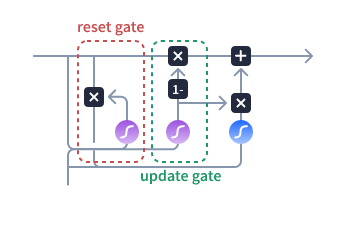
\includegraphics[scale=1]{Images/GRU_Architecture.png}
		\caption{GRU Architecture}
	\end{figure}

	Chúng ta có các công thức của GRU như sau: \\
	\begin{enumerate}
		\item Cổng reset: $r_t = \sigma(W_r \cdot [h_{t-1}, x_t])$
		\item Cổng update: $z_t = \sigma(W_z \cdot [h_{t-1}, x_t])$
		\item Ô nhớ hiện tại: $\tilde{h_t} = tanh(W \cdot [r_t \bigodot h_{t-1}, x_t])$
		\item Hidden state: $h_t = ( 1 - z_t ) \bigodot h_{t-1} + z_t \bigodot \tilde{h_t} $
	\end{enumerate}

	Dưới đây là cách mà GRU có thể giảm tác động của vanishing gradient:

	\begin{itemize}
		\item Cổng Update ($z_t$):
		Cổng update $z_t$ là nơi quyết định xem trạng thái trước đó $h_{t-1}$ sẽ được chuyển đến trạng thái hiện tại $h_t$ như thế nào. Khi $z_t$ gần bằng 1, nó cho phép thông tin được chuyển qua mà không cần thay đổi nhiều. Khi $z_t$ gần bằng 0, thì trạng thái mới $\tilde{h_t}$ quan trọng hơn nhiều. Vì vậy, kể cả khi $z_t$ gần bằng 0, gradient vẫn có thể đi qua cổng $z_t$ trong quá trình lan truyền ngược.
		\item Cổng Reset ($r_t$):
		Ngược lại, cổng reset $r_t$ kiểm soát trạng thái trước đó $h_{t-1}$ nên bị bỏ qua bao nhiêu khi tính toán $\tilde{h_t}$. Nếu $r_t$ gần bằng 0, nó cho phép model hoàn toàn bỏ qua trạng thái trước, từ đó học được các short-term dependencies một cách hiệu quả.
	\end{itemize}

	Sự phối hợp giữa cổng reset và update cho phép GRU update bộ nhớ một cách có chọn lọc, cho phép nó học cả short-term and long-term dependencies một cách hiệu quả hơn mạng RNN truyền thống.
\end{solution} 

\begin{problem}
	How does LSTM prevent the vanishing gradient problem ?
\end{problem}
\begin{solution}
	Long Short-Term Memory networks (LSTMs) được thiết kế để bao quát các long-term dependencies dùng trong dữ liệu dạng chuỗi. Để làm được điều này, LSTM sử hữu một thiết kế ô nhớ phức tạp hơn nhiều so với mạng RNN truyền thống. \\
	\begin{figure}[H]
		\centering
		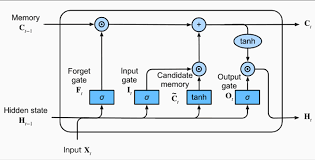
\includegraphics[scale=0.8]{Images/LSTM_Architecture.png}
		\caption{LSTM Architecture}
	\end{figure}
	Các thành phần quan trọng của LSTM bao gồm, \textit{cell state, input gate, forget gate} and \textit{output gate}:
	\begin{enumerate}
		\item Input Gate: $i_t = \sigma(W_i \cdot [h_{t-1}, x_t])$
		\item Forget Gate: $f_t = \sigma(W_f \cdot [h_{t-1}, x_t])$
		\item Cell State Update: $\tilde{C_t} = tanh(W_C \cdot [h_{t-1}, x_t])$
		\item Output Gate: $o_t = \sigma(W_o \cdot [h_{t-1}, x_t])$
		\item Hidden State Update: $h_t = o_t \bigodot tanh(C_t)$
	\end{enumerate}
	
	Dưới đây là cách mà LSTM có thể giảm bớt ảnh hưởng của vanishing gradient:
	\begin{itemize}
		\item Forget Gate($f_t$):
		Cổng Forget quyết định bao nhiêu phần của Cell State trước đó nên được giữ lại. Nếu $f_t$ gần bằng 1, LSTM sẽ giữ lại phần lớn cell state trước đó, cho phép ghi nhớ các long-term dependencies. Điều này hạn chế vanishing gradient bằng cách maintain thông tin suốt các time steps.
		\item Cell State Update ($\tilde{C_t}$):
		Cell này sẽ bao quát các thông tin mới từ input $x_t$, và hidden state trước đó $h_{t-1}$. Hàm activation \textit{tanh} đảm bảo rằng các giá trị sẽ được scaled để nằm trong khoản -1 và 1, từ đó việc lan truyền gradient sẽ trở lên dễ dàng hơn trong quá trình \textit{backpropagation}.
	\end{itemize}
\end{solution}

\end{document}
